\documentclass[twoside,12pt]{article}
\usepackage{amsmath,amsfonts,amsthm,fullpage,amssymb}
\usepackage{algorithm,hyperref}
\usepackage{algorithmic}
\usepackage{graphicx}
\usepackage{tcolorbox}
\usepackage{hyperref}

\begin{document}
\title{Notes on Neural Networks}
\author {Shasha Liao \\ Georgia Tech}
\maketitle
\section{"Expressive power" of Artificial Neural Networks}
\begin{itemize}
\item Can find a highly nonlinear decision boundary!
\item Every Boolean function can be represented by network with single hidden layer
\item Every bounded continuous function can be approximated with arbitrary small error by network with one hidden layer [Cybenko 1989; Hornik et al 1989]
\item Any function can be approximated to arbitrary accuracy by a network with two hidden layers. [Cybenko 1988] 
\item "Universal Approximator"
\end{itemize}
\section{ Logistic Regression: A simple Neural Network with one neuron}
\begin{itemize}
\item Model the conditional probability: $$\hat{y} = p(y=1|x,\theta) = \frac{1}{1+e^{-\theta^Tx}} = \sigma(\theta^Tx),$$ where $\sigma$ is the sigmoid function $\sigma(u) = \frac{1}{1+e^{-u}}$. 
\item Maximum log conditional likelihood: $$l(\theta) := \log\Pi_{i=1}^m p(y^i|x^i,\theta)  = \sum_{i=1}^m \log((\hat{y}^i)^{y^i}(1 - \hat{y}^i)^{1 -y^i}) = \sum_{i=1}^m (y^i\log \hat{y}^i + (1-y^i)\log(1- \hat{y}^i) ).$$
$l(\theta)$ is convex function, so it has a single global maximum. But there is no closed form solution. So we need to use iterative methods like gradient descent or stochastic gradient descent to find the global optimum.
\item Linear decision boundary: $$\log \frac{p(y=0|x)}{p(y=1|x)} = 0 \Longleftrightarrow  \theta^Tx = 0.$$
\end{itemize}

\section{Adding Nonlinearity: Nonlinear Neurons (Activation Functions)}
A good neuron should be bounded, easily differential, monotonic (good for convex optimization), and easy to handle.
\begin{itemize}
\item Hard limiter: $f(u) = \left\{ \begin{array}{lcr} 1, & \mbox{ if } & u \geq 0; \\ 0, & \mbox{ otherwise}.& \end{array} \right.$
\item Piecewise linear function: $f(u) = \left\{ \begin{array}{lcr} 1, & \mbox{ if } & u \geq 1; \\ u, &\mbox{ if }& u \in [0,1] \\ 0, & \mbox{ if } & u < 0. \end{array} \right.$
\item Sigmoid function: $\sigma(u) = \frac{1}{1+e^{-u}}$ \\
1, Has all the fundamental properties of a good activation function.\\
2, Take values between 0 and 1, good for modeling probability 
\item Hyperbolic tangent: $\tanh(u) = \frac{e^u - e^{-u}}{e^u + e^{-u}}$\\
1. Often found to converge faster in practice. \\
2. Gradient is easy to compute: $\tanh'(u) = 1- \tanh^2(u)$
3. Take values between -1 and 1, allows the state vector to increase and decrease.
\item Relu function: $f(u) = \max (u,0)$ \\
0. Very easy to compute. The most popular activation used today.\\
1. Can deal with vanishing gradient\\
2. Dose not saturate even for large values of $u$\\
3. Found with much success in computer vision \\
But \\
4. Suffer from \textit{dying ReLU problem} since neurons arriving at large negative values cannot recover from being stuck at 0. The network will stop learning and underperforms if the neurons are not initialized properly or when the data is not normalized very well.
\item Leaky Relu: $f(u) = \max (u,ku)$ with  $0 < k < 1$ small\\
1. $f'(u) = \left\{ \begin{array}{lcr} 1, & \mbox{ if } & u \geq 0; \\ k, & \mbox{ if } u < 0& \end{array} \right.$ \\
2. Solve the problem of \textit{dying ReLU problem}.
\item Relu with bias: $f(u, \theta) = \max(u+\theta, 0)$
\end{itemize}
\begin{center}
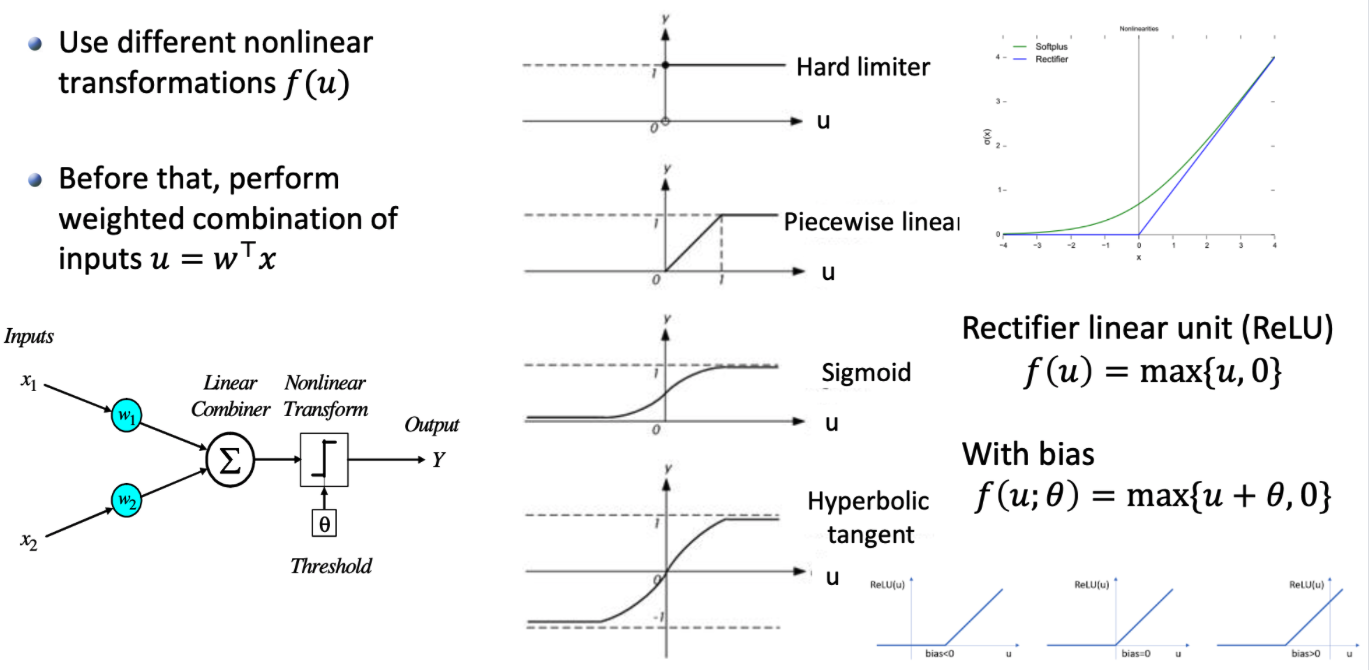
\includegraphics[width=0.95\textwidth]{activations.png}
\end{center}
\section{Multi-class Classification: Softmax function}
$$p(y^i = c| x^i) = \frac{\exp{\theta_c^T x^i}}{\sum_{c'} \exp{\theta_{c'}^T x^i}}$$

\section{Training neural networks: Backpropagation}
\begin{itemize}
\item Objective function: $$\min_{w,\alpha, \beta} l(w,\alpha, \beta) = \sum_{i = 1}^m (y^i - \sigma(w^Tz^i)).$$
\item Non-convex objective function.
\item Use chain rule to find the gradients for all the parameters.
\item Use gradient descent to find a local optimum. 
\item Different initialization may lead to different results.
\end{itemize}

\section{Classification performance measures}
\begin{itemize}
\item Mis-classification error: $$\frac{\# \text{mis-classified samples}}{\#\text{total}}$$
\item Confusion matrix: columns are actual classes and rows are predicted classes. Confusion matrix makes it easy for us to see what classes our model is struggling with. 
\item Precision and Recall: $$\text{Precision} = \frac{TP}{TP + FP} \quad \text{Recall} = \frac{TP}{TP + FN}$$
\begin{itemize}
\item Defined for each class. Imagine you look at all the images predicted to be cats. Then think about the following two questions. 
\item Precision: what proportion of positive identifications was actual positive? \\
Ex: what proportion of predicted cats are actually cats?
\item Recall: what proportion of actual positives was identified correctly? \\
Ex: what proportion of actual cats was identified correctly? 
\end{itemize}
\item F1 score: the harmonic average of precision and recall, taking values between 0 and 1. \\
$$\frac{1}{\text{F1}} = \frac 1 2 (\frac{1}{\text{Precision}} + \frac{1}{\text{Recall}}) .$$
We consider the harmonic mean of Precision and Recall because they have the same numerator. Moreover, if any one of them is small, the harmonic mean will also be small. In other words, the harmonic mean is large only when both Precision and Recall are large. This is different from the arithmetic mean where a large value and a small value will still lead to a pretty large mean. \\

Ex: A data set will 1 A and infinitely many Bs. The classifier predicts every data to be in class A. \\
This classifier has precision = 0 but recall = 1. \\
Arithmetic mean: 0.5. \\
Harmonic mean: 0.
\end{itemize}

\section{Common neural network structures}
\subsection{Supervised neural networks}
\begin{itemize}
\item Full connected neural networks: Not very practical. Easy to overfitting.
\item Convolutional neural networks: good for images; nodes in one layer are only locally connected to nodes in the next layer; two types of layers: convolution and max pooling
\item Recursive neural network: good for sequential / time series data; neural network structure repeats itself; attention mechanism (jump over time, take previous inputs, avoid forgetting important things earlier), transformer. 
\item Residual neural network: jump over some layers. 
\end{itemize}
\subsection{Unsupervised neural networks}
\begin{itemize}
\item GAN: Generative adversarial neural networks: better generator and better discriminator 
\item Auto-encoder: network learn to represent data itself
\end{itemize}

%\section{}
%\begin{itemize}
%\item
%\end{itemize}
\end{document}